\documentclass{article}
\usepackage[T1]{fontenc}
\usepackage{lmodern}
\usepackage{graphicx}
\usepackage{amsmath,amssymb}
\usepackage[a4paper,margin=2cm]{geometry}
\usepackage[absolute,overlay]{textpos}
\setlength{\TPHorizModule}{1mm}
\setlength{\TPVertModule}{1mm}
\usepackage[indonesian]{babel}
\usepackage{hyperref}
\setlength{\emergencystretch}{2em}
% unit: Halaman 28

\begin{document}

% === Halaman 28 (llm) ===

\vspace{139.59mm}

\section*{Diagram Proses Steganografi}
\vspace{40mm}

% deskripsi: Diagram alur proses steganografi yang menunjukkan langkah-langkah dari pesan rahasia (Embedded message) yang digabungkan dengan cover-object menggunakan encoder dan kunci (key) untuk menghasilkan stego-object, yang kemudian didekode oleh decoder menggunakan kunci untuk mengekstraksi kembali pesan rahasia. Terdapat juga elemen 'adversary' yang mencoba menganalisis stego-object tersebut.
% bbox normalisasi: [0.1600, 0.3100, 0.8700, 0.7800]
\begin{textblock*}{149.10mm}(33.60mm,92.07mm)
\noindent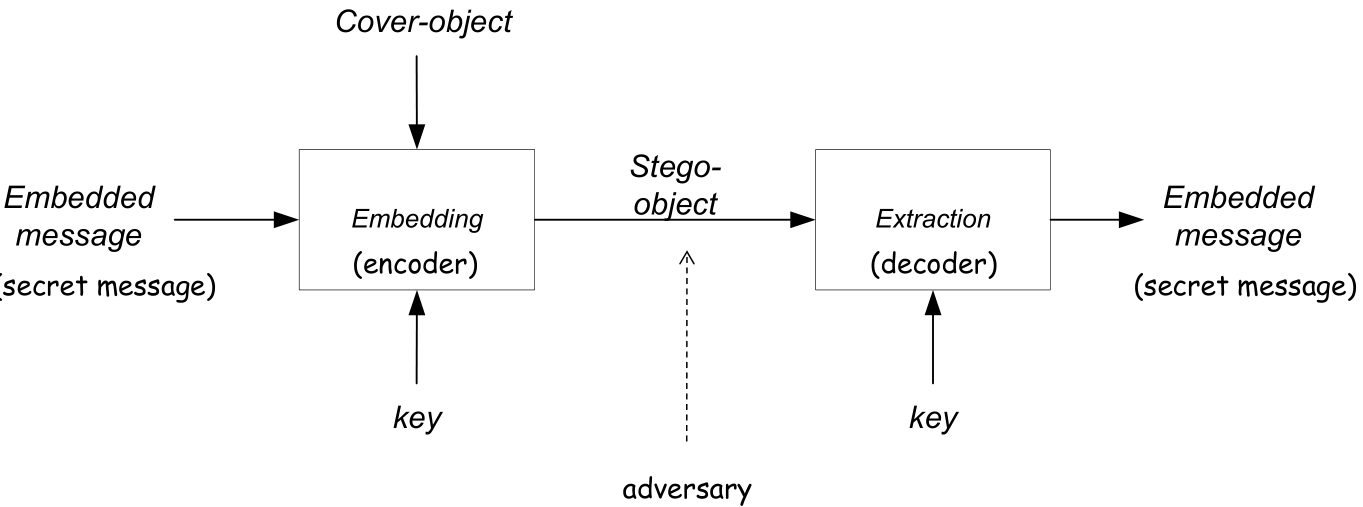
\includegraphics[width=149.10mm,height=139.59mm]{../../images/llm/page_028_img_01.png}%
\end{textblock*}

\end{document}
